\documentclass[12pt,oneside]{book}

\usepackage[dvips,letterpaper,margin=0.75in,bottom=0.75in]{geometry}
\usepackage{cite}
\usepackage{slashed}
\usepackage{graphicx}
\usepackage{amsmath}
\usepackage{enumitem}

\usepackage[american,fulldiode]{circuitikz}
\tikzset{component/.style={draw,thick,circle,fill=white,minimum size =0.75cm,inner sep=0pt}}

\begin{document}
\ctikzset{bipoles/thickness=1}
\ctikzset{bipoles/length=.6cm}

\title{Physics 80 Lab Manual}

\maketitle

\chapter{The Speed of Light in Air }

\section{Pre-lab Calculations}
\noindent
1) Suppose .  Hint: assume a . \\ 

\noindent
2)   \\

\noindent
3) What is the definition of the meter ? What is the exact value of the speed of light in vacuum?
%The meter  is the length of the path travelled by light in vacuum during a time interval of 1/299792458 second. The exact value for the speed of light in vacuum is 299,792,458 metres per second.

\section{Introduction}

In this lab, you will measure the speed of light in the air by measuring the time between sending and receiving a flash of light over a known distance, evaluate statistical and systematic uncertainties and compare it to the known value.  In the process, you will learn how to use your scope to make time measurement.

The flash of red light is created by a pulsed laser diode, a device very similar to a laser pointer, except this laser is switched on and off (pulsed) at a very high rate: 1 million times per second (1 MHz).  Whenever laser diode is pulsed a "trigger" pulse is sent to the oscilloscope. The pulsed beam of light is detected by a fast photo-diode detector and a "signal" pulse is sent to the oscilloscope. The time difference between the two pulses $\Delta t$ can be measured as a function of the distance $L$ between the laser/detector apparatus. 
Assuming that the time difference between the two pulses depends only on the time it took the light to travel the distance $L$ one can determine the  phase velocity of laser diode light in the air:   $v_{red}=\frac{L}{\Delta t}$.


%and the
%mirror
%can be bounced off of
%a mirror and the return pulses detected by a very responsive (“fast”) detector. Each pulse of the laser
%creates two signals, one from the laser itself (the “trigger”) and one from the detector when it picks up the
%returning pulse. These two signals can be compared to each other with a fast oscilloscope, and the time
%between them can be measured as a function of the distance between the laser/detector apparatus and the
%mirror. By varying the total distance from the laser to the detector L and monitoring the time difference
% on the scope, one can determine the speed of light c. If the time difference between the two signals 
%depended only on the time it took for the light to travel that distance, then c would be given by


\section{Measuring the $I$-$V$ Curve of a Diode}

In this section you will measure the $I$-$V$ curve of a 1N914 diode, and compare your results to the curves available from the device data sheet.  To avoid taking a bunch of measurements by hand, we will use a trick to plot the curve directly on your oscilloscope using the XY mode.
\begin{figure}[htbp]
\begin{center}
\begin{tabular}{c@{\hskip 2cm}c}

\begin{circuitikz}[line width=1pt]
\draw
(0,0) to[sinusoidal voltage source,bipoles/length=1.5cm,l=$\tilde{V}$] (0,4) -- (2,4);
\draw
(2,4) node[right]{$P_2$} to[resistor,l=$R_1$,o-o] (2,2) node[right] {$P_1$} to[diode,l=$D_1$,-o](2,0) node[right]{G}-- (0,0)
;
\draw (0,0) -- ++(0,0) node[ground,yscale=2.0]{};
\end{circuitikz} &

\begin{circuitikz}[line width=1pt]
\draw
(0,0) to[sinusoidal voltage source,bipoles/length=1.5cm,l=$\tilde{V}$] (0,4) -- (4,4);
\draw
(2,4) to[resistor,l_=$R_1$,*-o] (2,2) node[left]{$P_1$} node[right]{(Ch.1)} to[diode,l_=$D_1$,o-*] (2,0)
(4,4) to[diode,l=$D_2$,-o] (4,2) node[right] {$P_2$ (Ch.2)} to[resistor,l=$R_2$,-o](4,0) node[right]{G}-- (0,0)
;
\draw (2,0) -- ++(0,0) node[ground,yscale=2.0]{};
\end{circuitikz} \\
(a) & (b) \\
\end{tabular}
\caption{Diode circuits for (a) demonstrating rectification and (b) plotting the diode IV curve on your oscilloscope.}
\label{fig:diodecircuits}
\end{center}
\end{figure}

Consider (but don't build!) the circuit in Fig.~\ref{fig:diodecircuits}a.  The voltage between points $P_2$ and $P_1$ is proportional to the current passing through the diode, and the voltage between points $P_1$ and $G$ is the voltage across the diode.  So if we could display $P_2-P_1$ versus $P_1-G$ on your scope we could use this circuit.  Unfortunately, this is not possible on your scope, because (1) the only valid place to put the scope probe ground shield clips is at the point $G$ (Why?) and (2) you can only display Channel 1 versus Channel 2 in XY mode.   

The solution is to drive two copies of the diode in series resistor, with the component order reversed, as in Fig.~\ref{fig:diodecircuits}b.  This way, we can connect the probe ground shields as required at point $G$, put the voltage across the diode on scope Channel 1 by connecting the probe tip at $P_1$, and put the voltage across the resistor (proportional to current through the diode) on scope Channel 2 by connecting the probe tip at $P_2$.

Build the circuit in Fig.~\ref{fig:diodecircuits}b using a 1N914 fast switching diode for $D_1$ and $D_2$ and $R_1= R_2 = 10~{\rm k\Omega}$.  Set your function generator for high-impedance output, providing AC with peak to peak voltage of $20~\rm V$ at a frequency of $100~\rm Hz$.  Before switching to XY mode, make certain that your Channel 1 has no voltage offset (that is, zero voltage is located at the origin) or else your diode output voltage won't be calibrated properly in your output plot.   Once you set this, try not to adjust the offset of Channel 1 or you'll have to redo it!  To minimize noise, set the bandwidth limit ``On'' for both channels (this is available in the menu for each input channel as ``BW Limit'').

\begin{figure}[htbp]
\begin{center}
\begin{tabular}{c@{\hskip 2cm}c}
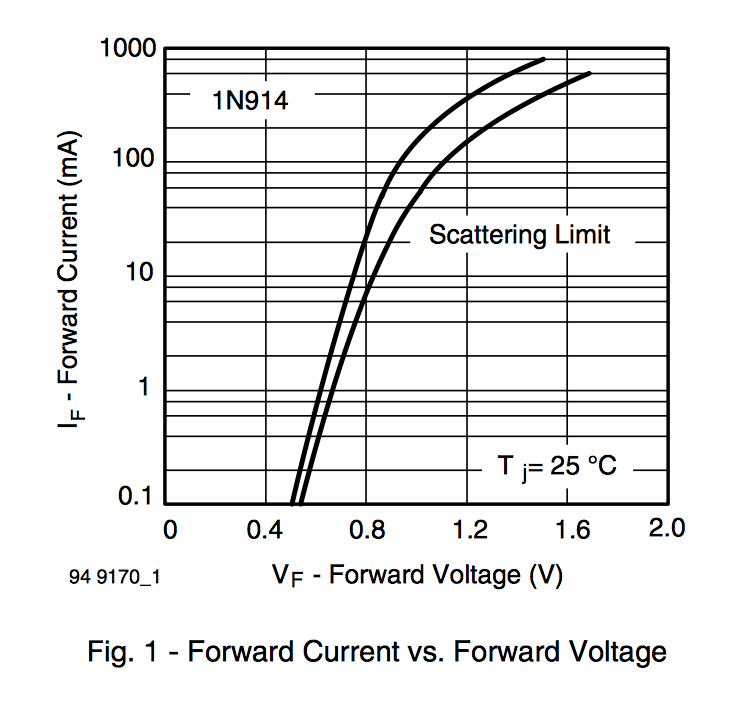
\includegraphics[height=0.25\textheight]{figs/labs/diode/1N914.png} &
\begin{picture}(200,100)
\put(0,0){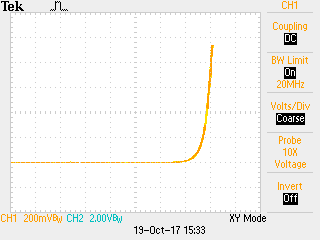
\includegraphics[height=0.25\textheight]{figs/labs/diode/diodeiv.png}}
\put(10,52){$0~mA$}
\put(10,70){$0.2~mA$}
\put(10,88){$0.4~mA$}
\put(10,106){$0.6~mA$}
\put(10,124){$0.8~mA$}
\put(10,142){$1.0~mA$}
\end{picture}\\
(a) & (b) \\
\end{tabular}
\caption{\label{fig:diodeiv} IV curves for the1N914 from (a) data sheet, and (b) as you will measure in this lab.  In the scope trace, the Channel 2 ($Y$) with scale set to $2~\rm V$ measures the voltage across a $10~\rm k\Omega$ resistor, so each division corresponds to $200~\rm \mu A$ as indicated. 
}
\end{center}
\end{figure}

Set the scope into XY mode, and see if you can reproduce the diode IV curve in Fig~\ref{fig:diodeiv}b.
Beats jotting down voltages in your logbook doesn't it?  Now jot down the voltage you expect across the diode for a current of $1~\rm mA$ in your logbook.  Where they overlap, does your measured IV curve agree with the curve from the component data sheet in Fig.~\ref{fig:diodeiv}a?

\section{Rectifying an AC Signal}

\begin{figure}[htbp]
\begin{center}
\begin{circuitikz}[line width=1pt]
\draw
(0,0) to[sinusoidal voltage source,bipoles/length=1.5cm,l=$\tilde{V}$] (0,4) -- (2,4)
(2,4) node[right]{$P_2$} to[diode,l=$D$,o-o] (2,2) node[right] {$P_1$} to[resistor,l=$R$,-o](2,0) node[right]{$G$} -- (0,0)
(2,0) -- ++(0,0) node[ground,yscale=2.0]{};
\end{circuitikz} 
\caption{A diode rectification circuit.}
\label{fig:rect}
\end{center}
\end{figure}

Set your function generator to provide an AC source with frequency $100~\rm Hz$ and peak-to-peak voltage $V_{\rm pp}=5~\rm V$.  Build the circuit in Fig.~\ref{fig:rect} using a 1N914 diode for $D$ and $R=1.8~\rm k\Omega$. 

With your scope probe ground shield clips both properly connected to the ground at $G$, monitor the voltage at points $P_1$ and $P_2$.   Sketch the voltage across the resistor $R$ and the voltage supplied by the function generator versus time on the same plot in your lab book. 

Using your scopes amplitude measurement feature, measure precisely (i.e. to within $50~\rm mV$ precision) the voltage drop across the diode at the peak current value, by measuring the difference between Channel 1 and Channel 2 of your scope at the peak.  Is this operating point consistent with your results from the previous section and the pre-lab calculations?


\section{Lab Report}

Your report should include all of your measurements and a comparison with your calculation.
 

\end{document}